\begin{question}{27}{
    Een tactisch hoofdkwartier analyseert het aantal vijandelijke drone-aanvallen dat op een bepaald veldhospitaal wordt uitgevoerd gedurende een periode van $24$ uur.

    Laat $X$ het aantal geregistreerde drone-aanvallen per dag zijn.
    Uit historische sensordata blijkt dat de kansverdeling van $X$ gemodelleerd kan worden met de volgende discrete kansfunctie:
    \begin{align*}
        p(k) = P(X = k) 
        \begin{cases}
            c \cdot \frac{2^k}{k!}, & \text{ voor } k = 0, 1, 2, 3, 4 \\
            0,                      & \text{ anders.}
        \end{cases}
    \end{align*}
}
    \subquestion{7}{
        Bereken de kansen $P(X = k)$ voor $k = 0,1,2,3,4$ in termen van de onbekende constante $c$.
        Toon daarna met deze kansen aan dat $p(k)$ voldoet aan de twee eisen van een goed gedefinieerde kansfunctie als $c = \frac{1}{7}$.        
    }
    \answer{
        Om deze kansfunctie in tabelvorm te schrijven, moeten we eerst bekijken wat de kansen zijn voor $k=0,1,2,3,4$:
        \begin{align*}
            P(X = 0) &= c \cdot \frac{2^0}{0!} = c \\
            P(X = 1) &= c \cdot \frac{2^1}{1!} = 2c \\
            P(X = 2) &= c \cdot \frac{2^2}{2!} = 2c \\
            P(X = 3) &= c \cdot \frac{2^3}{3!} = \frac{4}{3}c \\
            P(X = 4) &= c \cdot \frac{2^4}{4!} = \frac{2}{3}c \rubric{2}
        \end{align*}

        De twee eisen voor een goed gedefinieerde kansfunctie $p(k)$ zijn als volgt:

        \begin{description}
            \item \textbf{Voorwaarde 1:} voor iedere uitkomst $k$ geldt $p(k) = P(X = k) \geq 0$.\rubric{1}
            \item \textbf{Voorwaarde 2:} de som van kansen over alle mogelijke uitkomsten is gelijk aan $1$, oftewel
            \[
                \sum_{k} p(x) = 1.\rubric{1}
            \]
        \end{description}
        
        Aan de eerste voorwaarde wordt duidelijk voldaan indien de constante $c > 0$, aangezien de breuk $\frac{2^k}{k!}$ altijd een positief getal is voor $k=0,1,2,3,4$ (en bij overige waarden voor $k$ geldt $p(k) = 0$).\rubric{1}
        Aan de tweede voorwaarde wordt voldaan indien geldt:
        \begin{align*}
            1 = \sum_{k} p(k)   &= \sum_{k=0}^{4} c \cdot \frac{2^k}{k!} \\
                                &= c + 2c + 2c + \frac{4}{3}c + \frac{2}{3}c  \\
                                &= c \cdot 7.\rubric{2}
        \end{align*}
        De enige waarde van $c$ waarbij aan de vergelijking $7c = 1$ wordt voldaan, is $c = \frac{1}{7}$.\rubric{1}
    }
        
    \subquestion{6}{
        Teken een schets van de cumulatieve verdelingsfunctie (CDF) van $X$ op het interval $[-1, 5]$.
        Geef hierbij duidelijk aan wat de betekenis is van de assen.
        Gebruik vervolgens de grafiek om de mediaan van $X$ te bepalen.
    }
    \answer{
        De cumulatieve verdelingsfunctie $F(k) = P(X \leq k)$ van een discrete kansvariabele bepalen we door voor $k=0,1,2,3,4$ de kansen op te tellen op uitkomsten kleiner dan of gelijk aan $k$:

        \begin{center}
            \begin{tabular}{*{6}{c}}
                \toprule
                    $k$     & $0$ & $1$ & $2$ & $3$ & $4$ \\
                \midrule
                    $p(k)=P(X=k)$  & $\frac{1}{7}$ & $\frac{2}{7}$ & $\frac{2}{7}$ & $\frac{4}{21}$ & $\frac{2}{21}$ \\
                \midrule
                    $F(k)=P(X \leq k)$  & $\frac{1}{7}$ & $\frac{3}{7}$ & $\frac{5}{7}$ & $\frac{19}{21}$ & $1$ \rubric{2} \\ 
                \bottomrule
            \end{tabular} 
        \end{center}
        Bij een cumulatieve verdelingfunctie van een discrete kansvariabele hebben we dan te maken met een trapsgewijze grafiek, waarbij voor $k=0,1,2,3,4$ een verticale stap wordt gezet met hoogte $p(k)$:

        \begin{center}
            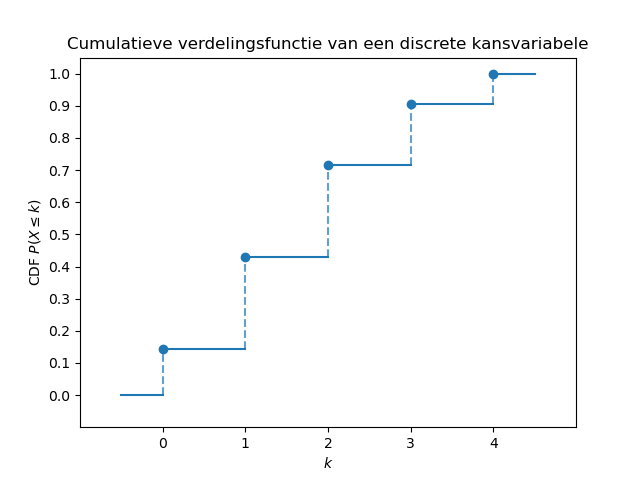
\includegraphics[width=0.5\textwidth]{./20261016_discrete_CDF.png} \rubric{4}
        \end{center}
    }


    \subquestion{8}{
        Bereken de verwachtingswaarde $E(X)$ en de standaardafwijking $\sigma(X)$ van het aantal geregistreerde drone-aanvallen $X$ per dag.
    }
    \answer{
        De verwachtingswaarde $E(X)$ berekenen we met behulp van de algemene formule:
        \begin{align*}
            E(X)    &= \sum_{k=0}^{4} k \cdot P(X=k) \\
                    &= 0 \cdot P(X=0) + 1 \cdot P(X=1) + 2 \cdot P(X=2) + 3 \cdot P(X=3) + 4 \cdot P(X=4) \\
                    &= 0 \cdot \frac{1}{7} + 1 \cdot \frac{2}{7} + 2 \cdot \frac{2}{7} + 3 \cdot \frac{4}{21} + 4 \cdot \frac{2}{21} \\
                    &= \frac{38}{21}.\rubric{3}          
        \end{align*}
        Om de standaardafwijking $\sigma(X)$ te berekenen, dienen we eerst de variantie $\Var{X}$ te berekenen:
        \begin{align*}
            \Var{X} &= \sum_{k=0}^{4} (k - E(X))^2 \cdot P(X=k) \\
                    &= (0 - E(X))^2 \cdot P(X=0) + (1 - E(X))^2 \cdot P(X=1) + (2 - E(X))^2 \cdot P(X=2) + (3 - E(X))^2 \cdot P(X=3) + (4 - \E(X))^2 \cdot P(X=4) \\
                    &= (0 - \frac{38}{21})^2 \cdot \frac{1}{7} + (1 - \frac{38}{21})^2 \cdot \frac{2}{7} + (2 - \frac{38}{21})^2 \cdot \frac{2}{7} + (3 - \frac{38}{21})^2 \cdot \frac{4}{21} + (4 - \frac{38}{21})^2 \cdot \frac{2}{21} \\
                    &\approx 1.3923. \rubric{3}
        \end{align*} 
        De standaardafwijking $\sigma(X)$ vinden we nu door de wortel uit de variantie te nemen:
        \begin{align*}
            \sigma(X) = \sqrt{\Var{X}} = \sqrt{1.3923} \approx 1.1800. \rubric{2}
        \end{align*}      
    }

    \subquestion{6}{
        De commandant van het tactisch hoofdkwartier moet noodmaatregelen treffen in het geval dat er in twee weken tijd minstens de helft van de dagen twee of meer drone-aanvallen plaatsvinden.
        Wat is de kans dat de commandant noodmaatregelen moet gaan treffen?
    }
    \answer{
        Introduceer een nieuwe variabele $Y$ die het aantal dagen (in twee weken) telt dat er minimaal twee drone-aanvallen plaatsvinden.
        De kans op minimaal twee drone-aanvallen op een willekeurige dag is
        \[
            P(X \geq 2) = 1 - P(X \leq 1) = 1 - \frac{3}{7} = \frac{4}{7}.\rubric{1}
        \]
        De variabele $Y$ is dus binomiaal verdeeld met $n = 14$ (aantal dagen in twee weken) en $p = \frac{4}{7}$. \rubric{2}

        De commandant gaat noodmaatregelen treffen als geldt dat $Y \geq 7$.\rubric{1}
        De kans hierop is gelijk aan
        \begin{align*}
            P(Y \geq 7) &= 1 - P(Y \leq 6) \\
                        &= 1 - \binomcdf(n=14, p=\frac{4}{7}, k=6) \\
                        &\approx 0.7918\rubric{2}
        \end{align*}
    }

\end{question}